%\documentclass{beamer}
\documentclass[RawSienna,dvipsnames]{beamer}

%%% Dichiarazione dei pacchetti standard.
\usepackage[italian]{babel}
\usepackage[utf8x]{inputenc}
\usepackage{eurosym}
%%% Personalizzazione del layout---articolata su cinque livelli.
%\usetheme{split}        % layout complessivo. 
%\usetheme{CambridgeUS}
\usetheme{AnnArbor}
\useinnertheme{rectangles} % layout interno.
\useoutertheme{infolines} % layout esterno.
\setbeamercolor{title}{fg=RawSienna}
\setbeamercolor{frametitle}{fg=RawSienna}
\usecolortheme{crane} % schema di colori.
\usefonttheme{professionalfonts}  % schema dei font.
\setbeamercolor{item}{fg=RawSienna}
% Inutile dire che se volete tutti i default, potete risparmiarvi gli ultimi
% quattro comandi. 
%%% Titolo e autore.
\title{Monolith}
\subtitle{An interactive bubble provider}
\author{Revisione di Qualifica}
%\institute{Gruppo Utilizzatoti Italiani di \TeX}
%\date{\today}
\date{29 agosto 2017}

\usepackage{listings}
\usepackage{color}
\definecolor{lightgray}{rgb}{.9,.9,.9}
\definecolor{darkgray}{rgb}{.4,.4,.4}
\definecolor{purple}{rgb}{0.65, 0.12, 0.82}

\lstdefinelanguage{JavaScript}{
  keywords={typeof, new, true, false, catch, function, return, null, catch, switch, var, if, in, while, do, else, case, break},
  keywordstyle=\color{blue}\bfseries,
  ndkeywords={class, export, boolean, throw, implements, import, this},
  ndkeywordstyle=\color{darkgray}\bfseries,
  identifierstyle=\color{black},
  sensitive=false,
  comment=[l]{//},
  morecomment=[s]{/*}{*/},
  commentstyle=\color{purple}\ttfamily,
  stringstyle=\color{red}\ttfamily,
  morestring=[b]',
  morestring=[b]"
}

\lstset{
   language=JavaScript,
   backgroundcolor=\color{lightgray},
   extendedchars=true,
   basicstyle=\footnotesize\ttfamily,
   showstringspaces=false,
   showspaces=false,
   numbers=left,
   numberstyle=\footnotesize,
   numbersep=9pt,
   tabsize=2,
   breaklines=true,
   showtabs=false,
   captionpos=b
}



\begin{document}
	
\begin{frame}
	\begin{center}
		
\includegraphics[scale=0.13]{img/obelix.png}
		\qquad\qquad
		
\includegraphics[scale=0.13]{img/monolith.png}
	\end{center}
	\titlepage
\end{frame}


\section[Sommario]{}
\begin{frame}
	\tableofcontents
\end{frame}	

\section{Il gruppo Obelix}
\begin{frame}
	
	\begin{columns}
		\begin{column}{0.2\textwidth}
			
		\end{column}
		
		\begin{column}{0.4\textwidth}
			\begin{itemize}
				\item Emanuele Crespan
				\item Tomas Mali
				\item Silvio Meneguzzo
				\item Nicolò Rigato
				\item Riccardo Saggese
				\item Federica Schifano
			\end{itemize}
		\end{column}
		
		\begin{column}{0.2\textwidth}
			
		\end{column}
	\end{columns}
	
	
\end{frame}

\section{Utilizzo SDK}
\begin{frame}
  \frametitle{Hello Bubble - How to}
  %[caption=My Javascript Example]
  \begin{center}
    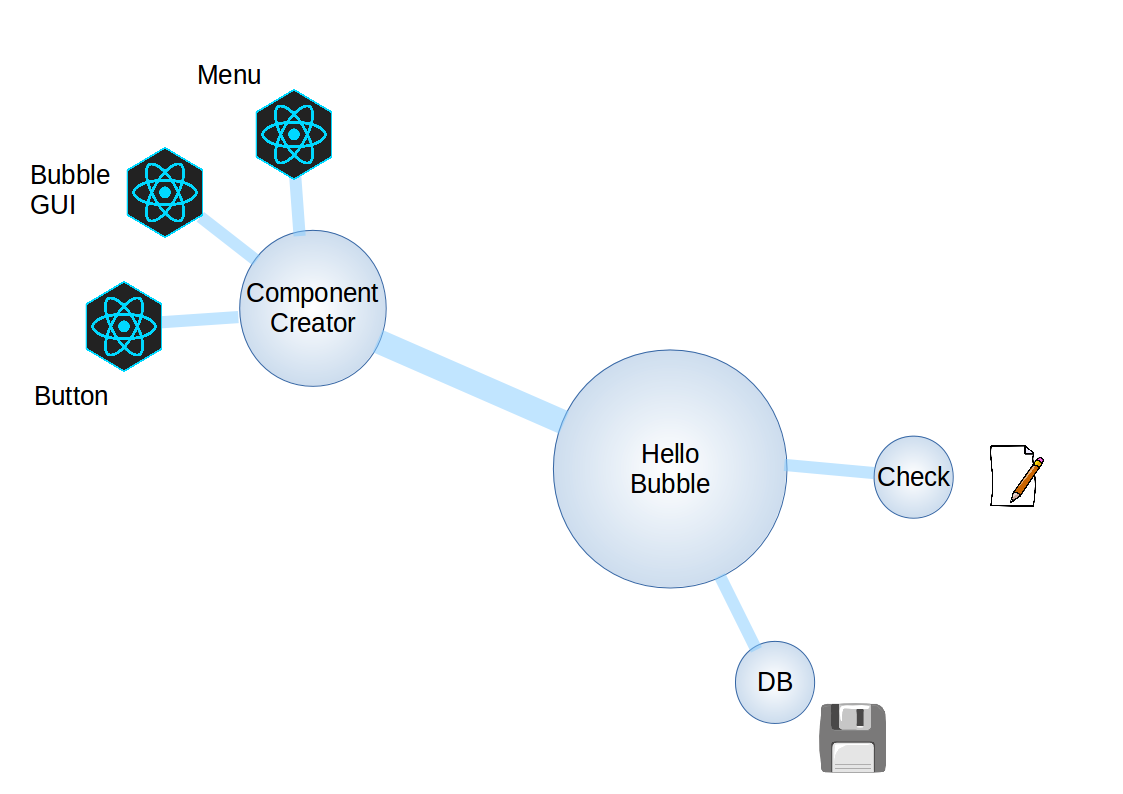
\includegraphics[scale=0.30]{code/bubbleMap.png}
  \end{center}
\end{frame}

\subsection{Hello Bubble - Gui}
\begin{frame}[fragile]
  \frametitle{Bubble Menu}
  %[caption=My Javascript Example]
  \begin{minipage}{.65\textwidth}
      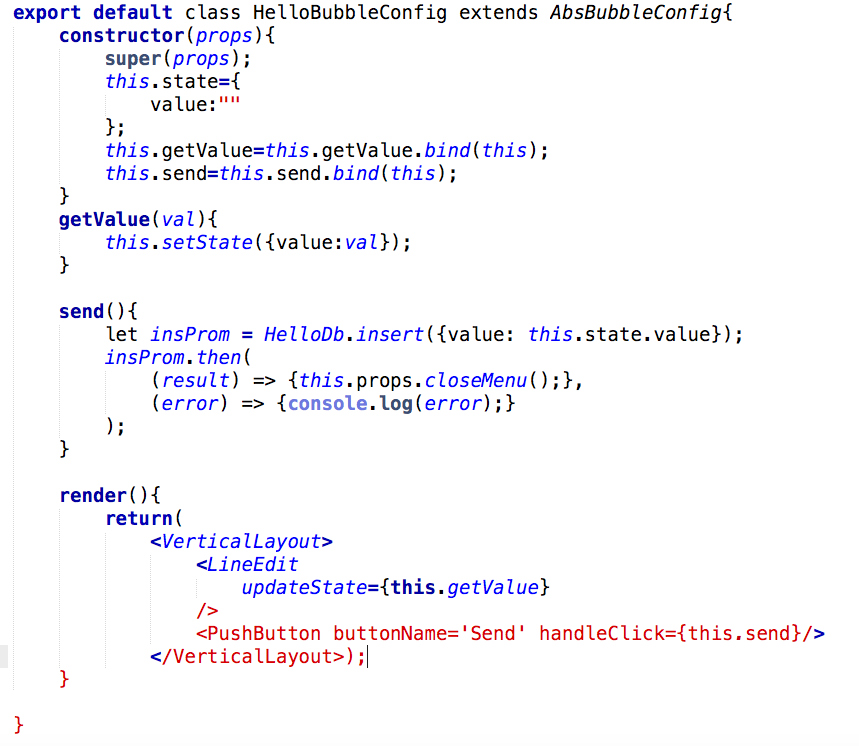
\includegraphics[width=\textwidth]{code/hellobubbleconfig.png}
  \end{minipage}
  \begin{minipage}{.34\textwidth}
      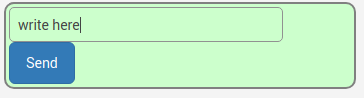
\includegraphics[width=\textwidth]{code/config.png}
  \end{minipage}
\end{frame}

\begin{frame}
  \frametitle{Bubble Button}
  %[caption=My Javascript Example]
  \begin{center}
  \begin{minipage}{.70\textwidth}
    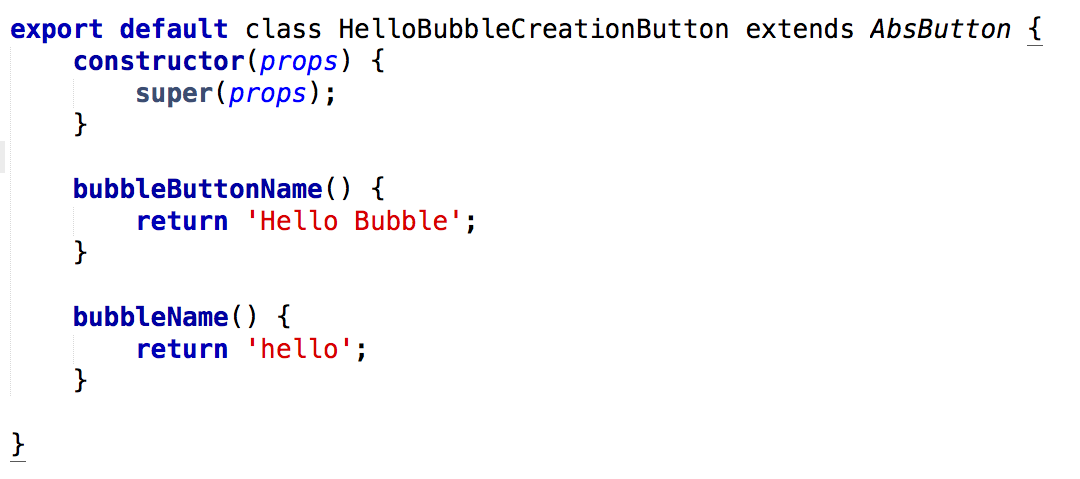
\includegraphics[width=\textwidth]{code/hellobubblecreationbutton.png}
  \end{minipage}
  \begin{minipage}{.28\textwidth}
    
\includegraphics[width=\textwidth]{code/button.png}
  \end{minipage}
  \end{center}
\end{frame}

\begin{frame}
  \frametitle{Bubble Gui}
  %[caption=My Javascript Example]
  \begin{center}
  \begin{minipage}{.65\textwidth}
    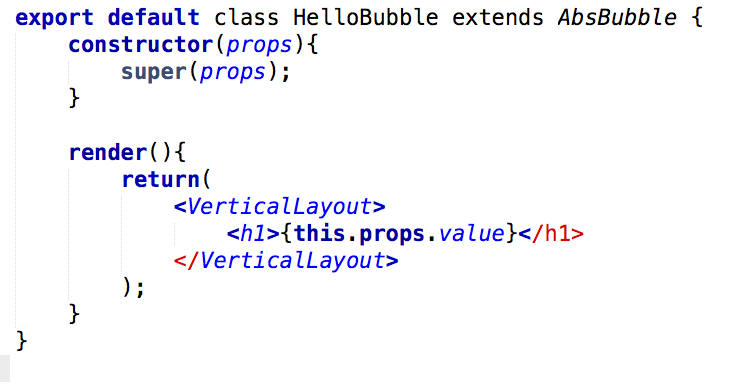
\includegraphics[width=\textwidth]{code/hellobubble.png}
  \end{minipage}
    \begin{minipage}{.34\textwidth}
    
\includegraphics[width=\textwidth]{code/bubble.png}
  \end{minipage}
  \end{center}
\end{frame}


\begin{frame}
  \frametitle{Gui managment}
  %[caption=My Javascript Example]
  \begin{center}
    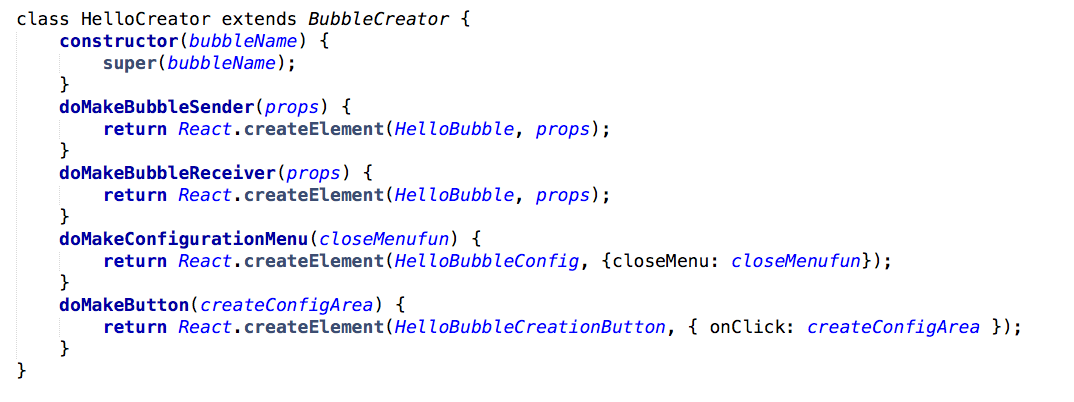
\includegraphics[width=.9\textwidth]{code/hellocreator.png}
  \end{center}
\end{frame}


\subsection{Database and data check}

\begin{frame}
  \frametitle{Database}
  %[caption=My Javascript Example]
  \begin{center}
    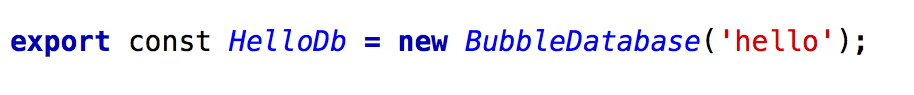
\includegraphics[width=.8\textwidth]{code/helloDb.png}
  \end{center}
\end{frame}

\begin{frame}
  \frametitle{Bubble Check}
  %[caption=My Javascript Example]
  \begin{center}
    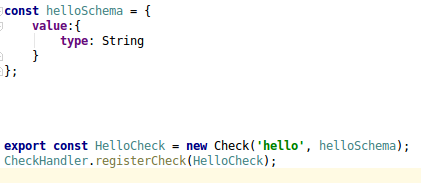
\includegraphics[width=.8\textwidth]{code/hellocheck.png}
  \end{center}
\end{frame}
 

\end{document}
